\chapter{Initial system design}
In this chapter I'm introducing the initial design of the above mentioned system from both hardware and
software aspects. Since there are several unknown factors 
during this phase, the designs described in this chapter represent an initial or starting step. The actual
system design will be based on the experience gained during several trial-and-error based iterations
in simulations.



\section{Simulation}
Before actually building the system and experimenting on an expensive quadcopter in real world environment,
it is cheaper, safer and easier to do tests in a simulated environment. 

The PX4 Firmware repository\cite{PX4Repository} contains Gazebo simulation files to give developers a head 
start in simulation of their product. Upon these simulation quadcopter models LIDAR sensors can be placed and 
moved around with ease, without the need of wiring or external infrastructure. This simulation is 
suitable for Software in the loop (SITL) testing, meaning that the same software developed for the simulation
can be used on a real quadcopter.



\subsection{Robot Operating System}
Robot Operating system (ROS) is a set of software libraries and tools that help developers to build robust 
general-purpose robot applications\cite{ROSWebsite}. ROS provides hardware abstraction of the underlying 
robot, generalizes the interfacing of these robots and allows simple high-level usage.


The core component of ROS is a public-subscribe communication protocol similar to MQTT protocol
used on the field of IoT. The ROS system is comprised of a number of independent communicating parties called 
nodes. Each node can subscribe to multiple topics and receive a stream of messages published to these topics 
by other nodes. For example a temperature filter node might subscribe to a topic of "/temperature\_sensor" 
and publish the filtered temperature values to a topic called "/filtered\_temperature\_sensor". 
The benefit using this solution is that the nodes achieve communication exclusively via this protocol 
so each node lives independently from another. Nodes in ROS do not need to be on the same system or 
even on the same architecture. Nodes can be run on different computers or even on microcontrollers or 
smartphones making the system flexible.

\begin{figure}[!ht]
    \centering
    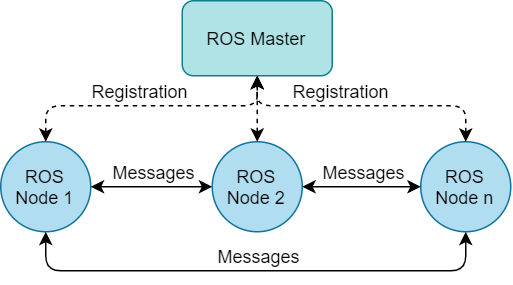
\includegraphics[width=100mm, keepaspectratio]{figures/ros_pubsub.png}
    \caption{ROS publish subscribe communication}
    \label{fig:ros_pubsub}
\end{figure}

To start a ROS session, a ROS Master needs to be started first. After starting the master, nodes can be 
started and each one registers the topics it wants to subscribe/publish to. The master handles these requests
and helps the nodes to establish connection between each other so communication can be started. 

ROS is language independent so nodes can be implemented in different programming languages. While C++ is 
the most common language for product development, official Python wrappers can be used for fast 
prototyping.


\subsection{Gazebo Simulator}
Gazebo\cite{GazeboWebsite} is an open-source 3D simulator for robotics, with the ability to accurately simulate robots in complex
indoor or outdoor environments. It is similar to game engines, but produces more realistic, physically correct
behavior. Gazebo is free, open-source, actively developed and has gained high popularity during the last years. 

Gazebo comes with a growing number of robots and sensors. For simulations one can choose from the officially 
available robots or create a custom robot using SDF files. Any of these robots can be customized and any 
number of sensors can be added. Using simulations sensor data can be generated and development can be started 
without having the actual hardware.

\begin{figure}[h]
    \centering
    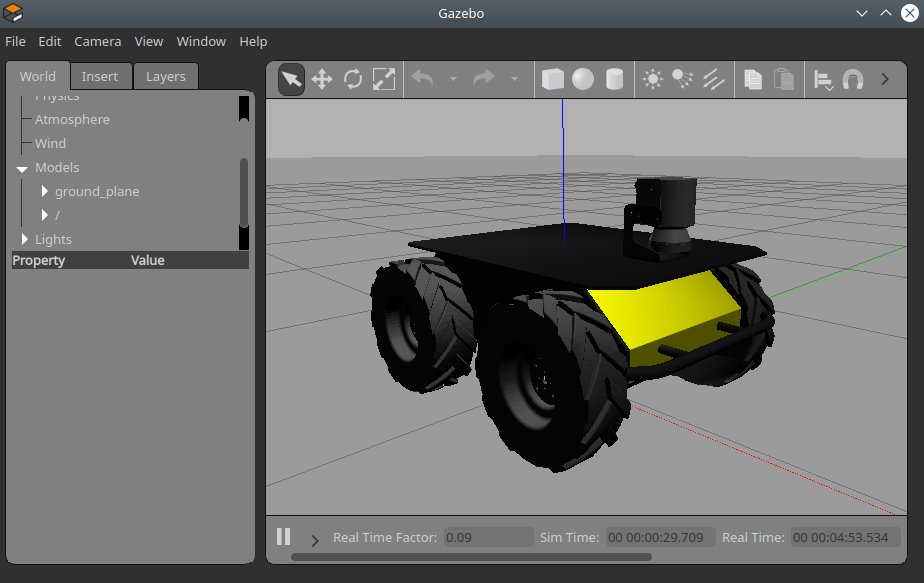
\includegraphics[width=100mm, keepaspectratio]{figures/husky.png}
    \caption{Gazebo ROS Husky robot demo}
    \label{fig:ros_husky}
\end{figure}

Why Gazebo is particularly interesting, is because it can be started in a ROS compatible mode. Gazebo
started with ROS wrapper will actively channel all sensor readings, states and many more to ROS topics, 
allowing nodes outside of the simulation to subscribe and publish to these topics. Using this technique nodes 
can be developed in a truly hardware independent manner. The simulation can be replaced by a real robot
and the nodes developed during this phase can be used without changes on the real hardware. For example a 
Husky robot can be simulated in Gazebo and controlled through ROS. The Gazebo simulation of a Husky 
can be seen on figure \ref{fig:ros_husky}.


\subsection{PX4 Autopilot Software}
PX4 is a powerful open-source autopilot flight stack. PX4 can control many different vehicle frames and types,
supports wide variety of sensors and peripherals. The project is a part of Dronecode, a nonprofit foundation
working on open-source projects to achieve standardization of drones.\cite{PX4Website} 

The core component of PX4 is the flight controller that controls the motors based on sensor measurements 
and executes commands received from ground control.


The PX4 Repository contains simulation files for Gazebo with many kind of vehicles. Using the simulator 
the same PX4 flight code can run on a computer modelled drone that would run on a real vehicle. The models can
be further extended by sensors or other peripherals, by modifying the SDF model files. SDF files are 
based on XML format, that makes them humanly readable and easy to modify using a text editor. 

The basic outline of the PX4 Software in the loop simulation can be seen on figure \ref{fig:px4_sitl_simulation}.



\begin{figure}[h]
    \centering
    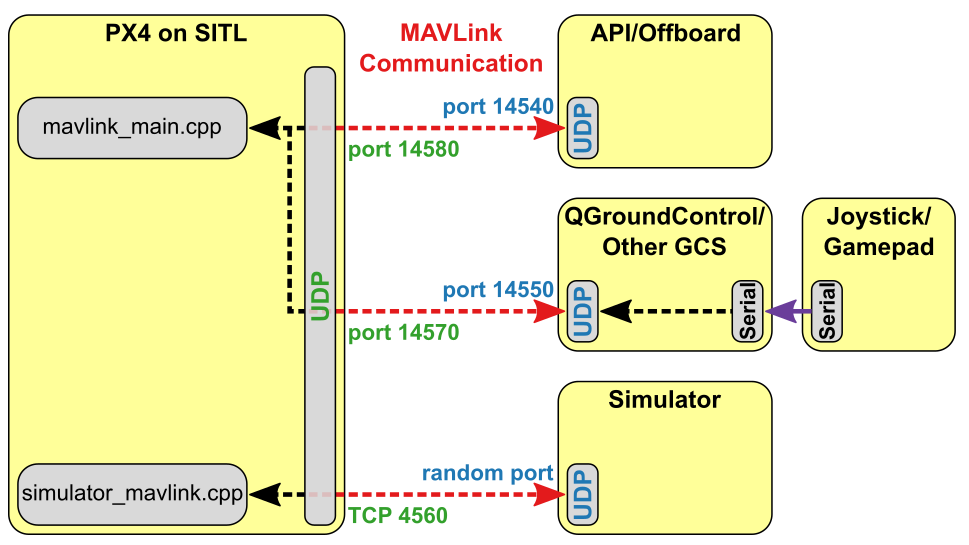
\includegraphics[width=120mm, keepaspectratio]{figures/px4_sitl_overview.png}
    \caption{PX4 SITL Simulation Outline \cite{PX4Simulation}}
    \label{fig:px4_sitl_simulation}
\end{figure}



\newpage
\section{Hardware plan}
\subsection{VL53L1X LIDAR}
\subsection{LIDAR placement}
\subsection{LIDAR data collection}
\subsubsection{Logging on SD Card}
\subsubsection{Wireless transceiver}
\subsubsection{Integrating messages into PX4 firmware}

\section{Software plan}